\begin{figure}[ht]
\centering
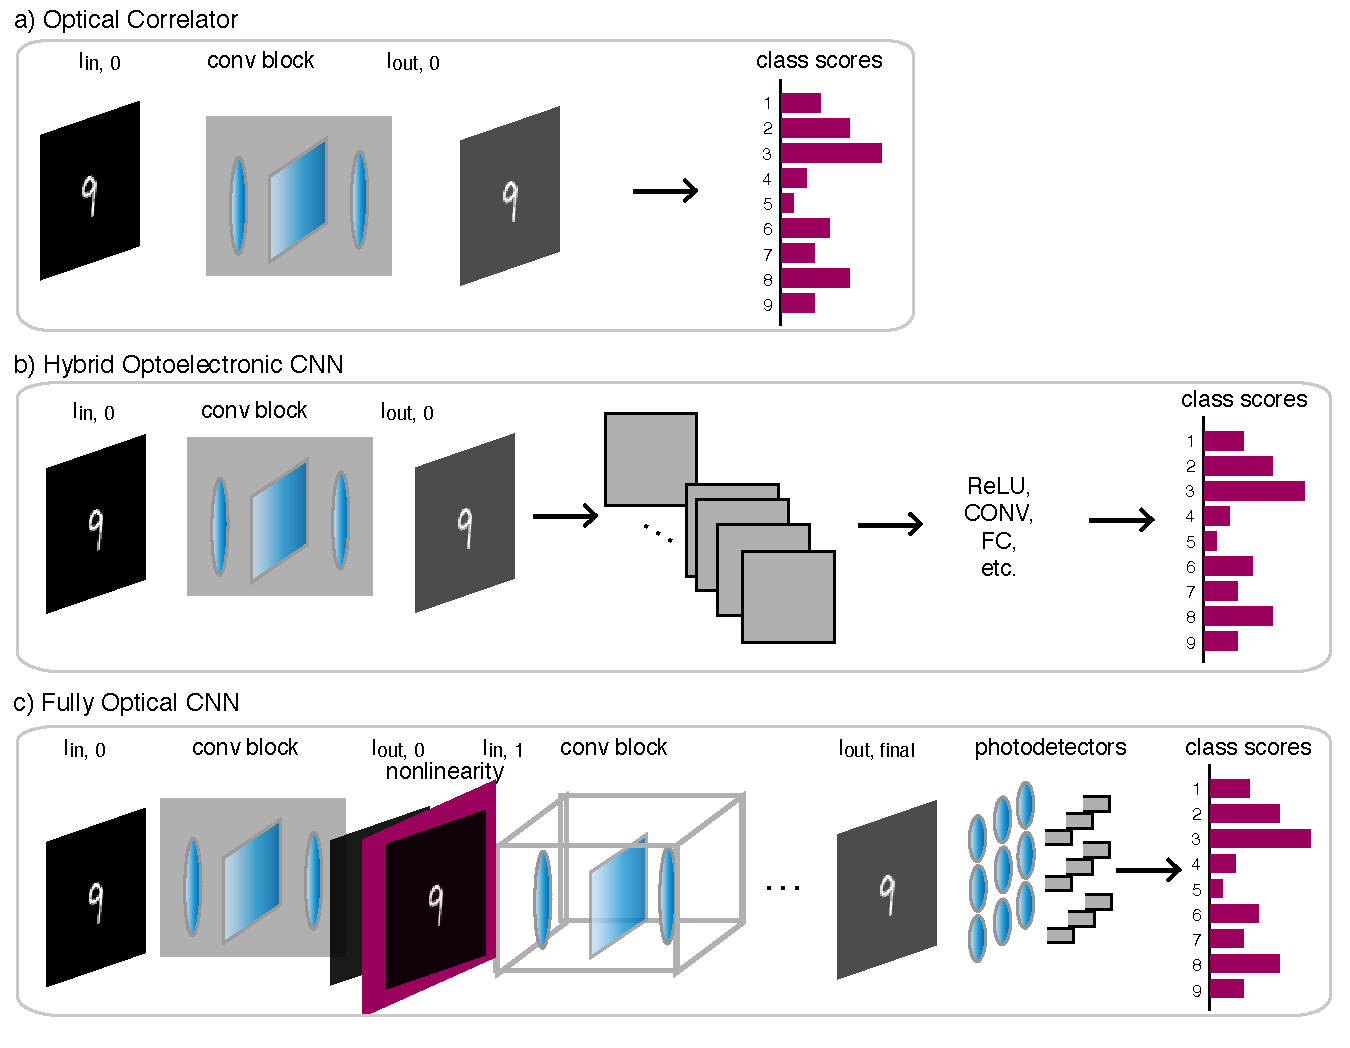
\includegraphics[width=\linewidth]{configs.pdf}
\caption{Optical classifier configurations. a) The optical correlator consists of a single optical convolutional layer. b) The hybrid optoelectronic CNN consists of one optical convolutional layer followed by one or more electronic CNN layers. c) The fully optical CNN is envisioned as a cascade of optical convolutional layers with nonlinear activation layers sandwiched between. }
\label{fig:configs}
\end{figure}

We build three convolution-based classifiers in simulation to better understand the performance of our optical CNN building blocks. We train these models to classify images from either the Google QuickDraw (PNG version) or CIFAR-10 dataset. Below we detail the setups and insights from each model. 

%%%%%%%%%%%%%%%%%%%%%%%%%%%%%%%%%%%%%%%%%%

\subsection*{Learned Optical Correlator}

\begin{figure}[ht]
\centering
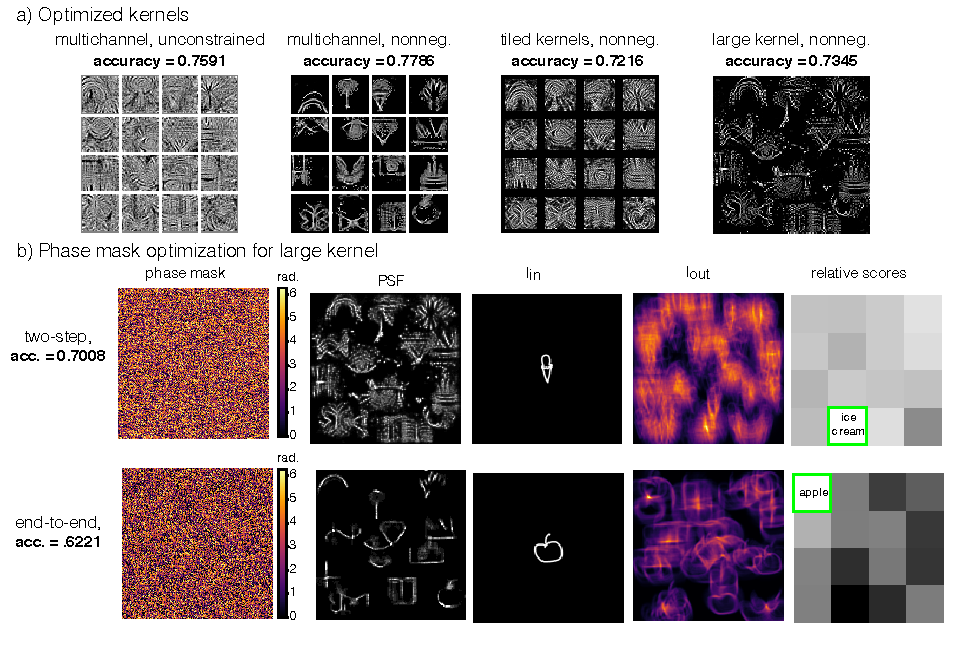
\includegraphics[width=\linewidth]{sim1.pdf}
\caption{Optical correlator. a) Characteristic optimized kernels of a multichannel unconstrained Tensorflow convolutional layer, a multichannel nonnegative Tensorflow convolutional layer, a single channel optical convolutional layer with tiled kernels, and a single channel optical convolutional layer with a freeform large kernel. b) Optimized phase masks corresponding to the large kernel.}
\label{fig:sim1}
\end{figure}

For our first experiment, we simulated a system with a single optical convolutional layer to confirm that our proposed optical convolution layer would function as expected. With a single convolutional layer, we expect to learn an optical correlator, which essentially performs template matching of the input image with the learned PSF. Here we are also able to apply end-to-end learning successfully (Fig. \ref{fig:sim1}b).

While this was interesting, an optical correlator is not powerful enough for more difficult classification tasks, for example with natural images or with more categories (see Supplement for the same experiment with CIFAR-10 images). Furthermore, at this point with a single layer, we still only have a linear classifier.

%%%%%%%%%%%%%%%%%%%%%%%%%%%%%%%%%%%%%%%%%%

\subsection*{Hybrid optoelectronic CNN} 
\begin{figure}[ht]
\centering
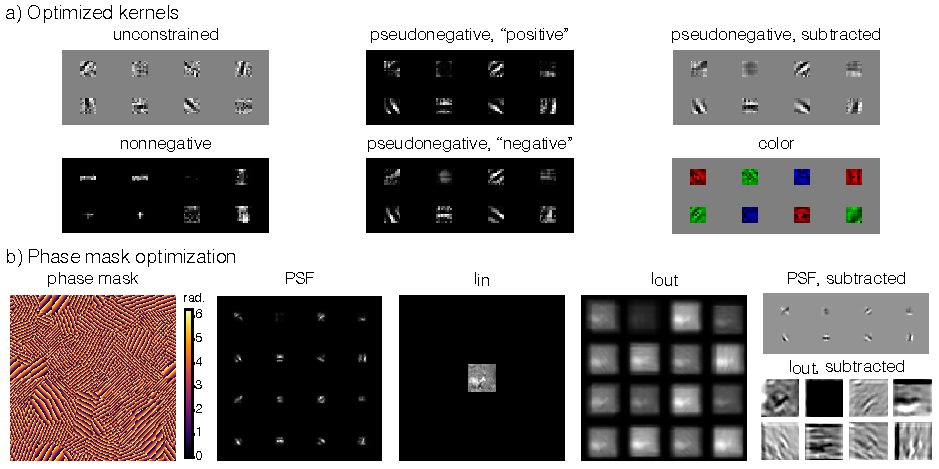
\includegraphics[width=\linewidth]{sim2.pdf}
\caption{Hybrid optoelectronic CNN}
\label{fig:sim2}
\end{figure}

Next we keep one optical convolutional layer but connect the output image to further electronic computations. This allows the first layer to be performed at zero input power. We do this with grayscale CIFAR-10 images.

\subsubsection*{Pseudo-negative weights}
Talk about the dual channel positive and negative weights. \\
When we attempted end-to-end optimization, we found that the optical element learned to simply replicate the input image (i.e. the PSF was a single point), so the fully connected layer was responsible for all the computation. 

\subsubsection*{Color filters - Vincent}
Alternatively, chromatic aberrations can be harnessed to encode color, so it would be interesting to explore multicolor masks as demonstrated in \cite{shechtman2016multicolour}.

\setlength{\tabcolsep}{4pt}
\begin{table}
\begin{center}
\caption{Classification accuracies on the grayscale CIFAR-10 dataset. Accuracies are the average of five trials.}
\label{table:hybrid}
\begin{tabular}{ l | c} 
 \textbf{Method} &  \textbf{Accuracy} \\ \hline \hline
FC				& 0.2982	\\
conv $>$ FC, unconstrained 	& 0.5186	\\
conv $>$ FC, nonnegative	 & 0.3632	 \\
conv $>$ FC, pseudonegative & 0.5176	\\
optical conv $>$ FC, pseudonegative & 0.4142	\\
optical conv $>$ FC, pseudonegative, refined 	& 0.5096
\end{tabular}
\end{center}
\end{table}
\setlength{\tabcolsep}{1.4pt}


%%%%%%%%%%%%%%%%%%%%%%%%%%%%%%%%%%%%%%%%%%

\subsection*{Fully optical CNN} 

The next goal was to create a fully optical CNN by incorporating additional optical convolutional layers with nonlinearity layers sandwiched in between. This doesn’t fully work, but can discuss some results.

\begin{figure}
\centering
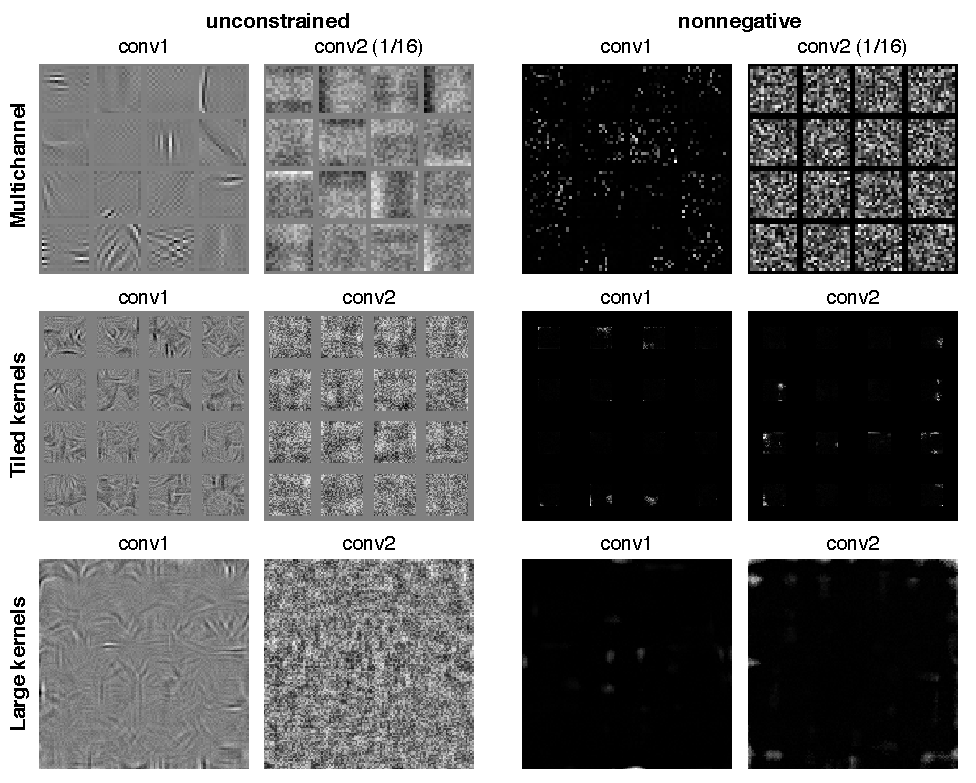
\includegraphics[width=\linewidth]{sim3.pdf}
\caption{Variations leading to a fully optical CNN.}
\label{fig:prototype}
\end{figure}


\setlength{\tabcolsep}{4pt}
\begin{table}
\begin{center}
\caption{Classification accuracies with various two-layer networks on 16 classes of the QuickDraw dataset. Accuracies are the average of five trials.}
\label{table:fullyoptical}
\begin{tabular}{ l | c | c  } 
 \textbf{Method} &  \textbf{Unconstrained} &  \textbf{Nonnegative}  \\ \hline 
multichannel (16)				& 0.810 & 0.810 \\
tiled kernels (16) 	& 0.8575	 & \\
large kernel	 & 0.3632	 & \\
\end{tabular}
\end{center}
\end{table}
\setlength{\tabcolsep}{1.4pt}